\chapter{Versuchsaufbau}

\section{Einleitung}

Um die vom Team erstellte Plattform auch unter realen Bedingungen testen zu können, wurde ein Versuchsaufbau mit zwei Drohnen erstellt, die es ermöglichen Produkte zu transportieren und über dem Kunden mit einem Fallschirm abzuwerfen. Der Aufbau der Drohnen beinhaltete die Zusammenstellung der passenden Komponenten, den Zusammenbau der Drohnen und die Planung und Erstellung von zusätzlichen Halterungen für die obengenannten spezifischen Anforderungen.\\

Bei der Zusammenstellung der Komponenten haben wir vor allem auf die gute Verfügbarkeit von Ersatzteilen und einen hohen Marktanteil der Komponenten geachtet. Besonders wichtig erschien uns, dass ein Anbieter nicht an einen Hersteller gebunden ist, sondern die Drohne an seine Bedürfnisse (Zuladung, Reichweite, Geschwindigkeit) anpassen kann. Es sollten also möglichst wenige Vorraussetzungen bestehen um die Plattform nutzen zu können, folgende sind allerdings unabdingbar:

\begin{itemize}

\item Flight-Controller muss \Gls{MAVLink} Protokoll unterstüzen
\item Onboard-App muss über MAVLink mit dem Flight-Controller verbunden sein. (Über USB oder eine Funk-Telemetrieverbindung.)
\end{itemize}

Im folgenden Kapitel werden die Komponenten und deren Eigenschaften genauer untersucht und beschrieben, wie auch die Möglichkeiten zur Verwendung von anderer Hardware- und Software auf dem Copter genauer erläutert.

\section{Multicopter Hardware}

\subsection{Frame und Antrieb}

Der Frame, die Motoren und ESCs wurden als Kit gekauft. Es handelt sich dabei um ein DJI Flamewheel 450 Frame mit DJI 2312 960kV Motoren und ESeries 420 20A ESCs. Dieses Kit ist weltweit gut verfügbar und deshalb ideal geeignet um einen Versuchsaufbau zu erstellen.

\begin{figure}[h]
\centering
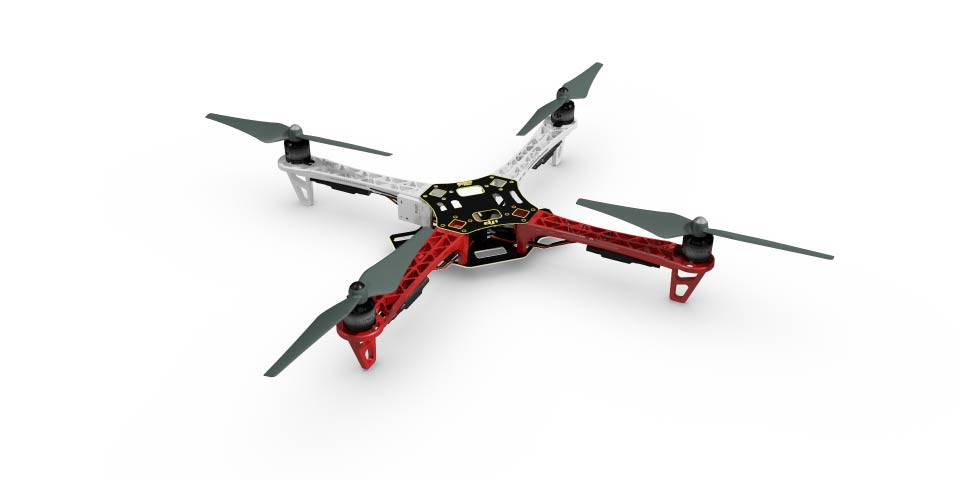
\includegraphics[width=0.9\textwidth] {images/hardware/f450.jpg} 
\caption{DJI F450 Flamewheel Kit}
\label{fig:f450}
\end{figure}


\subsection{Flight-Controller}

Der Flight-Controller ist das Herzstück eines Quadcopters. Im Unterschied zu anderen ferngesteuerten Fahr- und Flugzeugen kann ein Multicopter nur über ein Fly-by-Wire System kontrolliert werden. Das heisst alle Befehle, die von der Fernbedienung gesendet werden, müssen interpretiert und umgewandelt werden, damit die Motoren eine Bewegung in die gewünschte Richtung erzeugen können. In Kombination mit einem GPS Modul (Abb. \ref{fig:gps-module}) ermöglich der Controller verschiedene Flugmodi, wie beispielsweise das Schweben an einem Punkt oder automatisches abfliegen von Wegpunkten.

Als Flight-Controller setzen wir ein Pixhawk ein. Es ist sehr vielseitig und kann gut mit zusätzlichen Sensoren erweitert werden, ausserdem unterstützt es gängige Firmwares, die auch auf günstigeren Controllern laufen. Als Firmware für das Pixhawk setzen wir ArduCopter ein, da sie komplett Open-Source ist und auch bei vielen anderen Projekten eingesetzt wird. Sie unterstützt ausserdem das \Gls{MAVLink} Protokoll, das es ermöglicht verschiedene Flight-Controller über verschiedene Protokolle und Anschlüsse anzusprechen.

\begin{figure}[h]
\centering
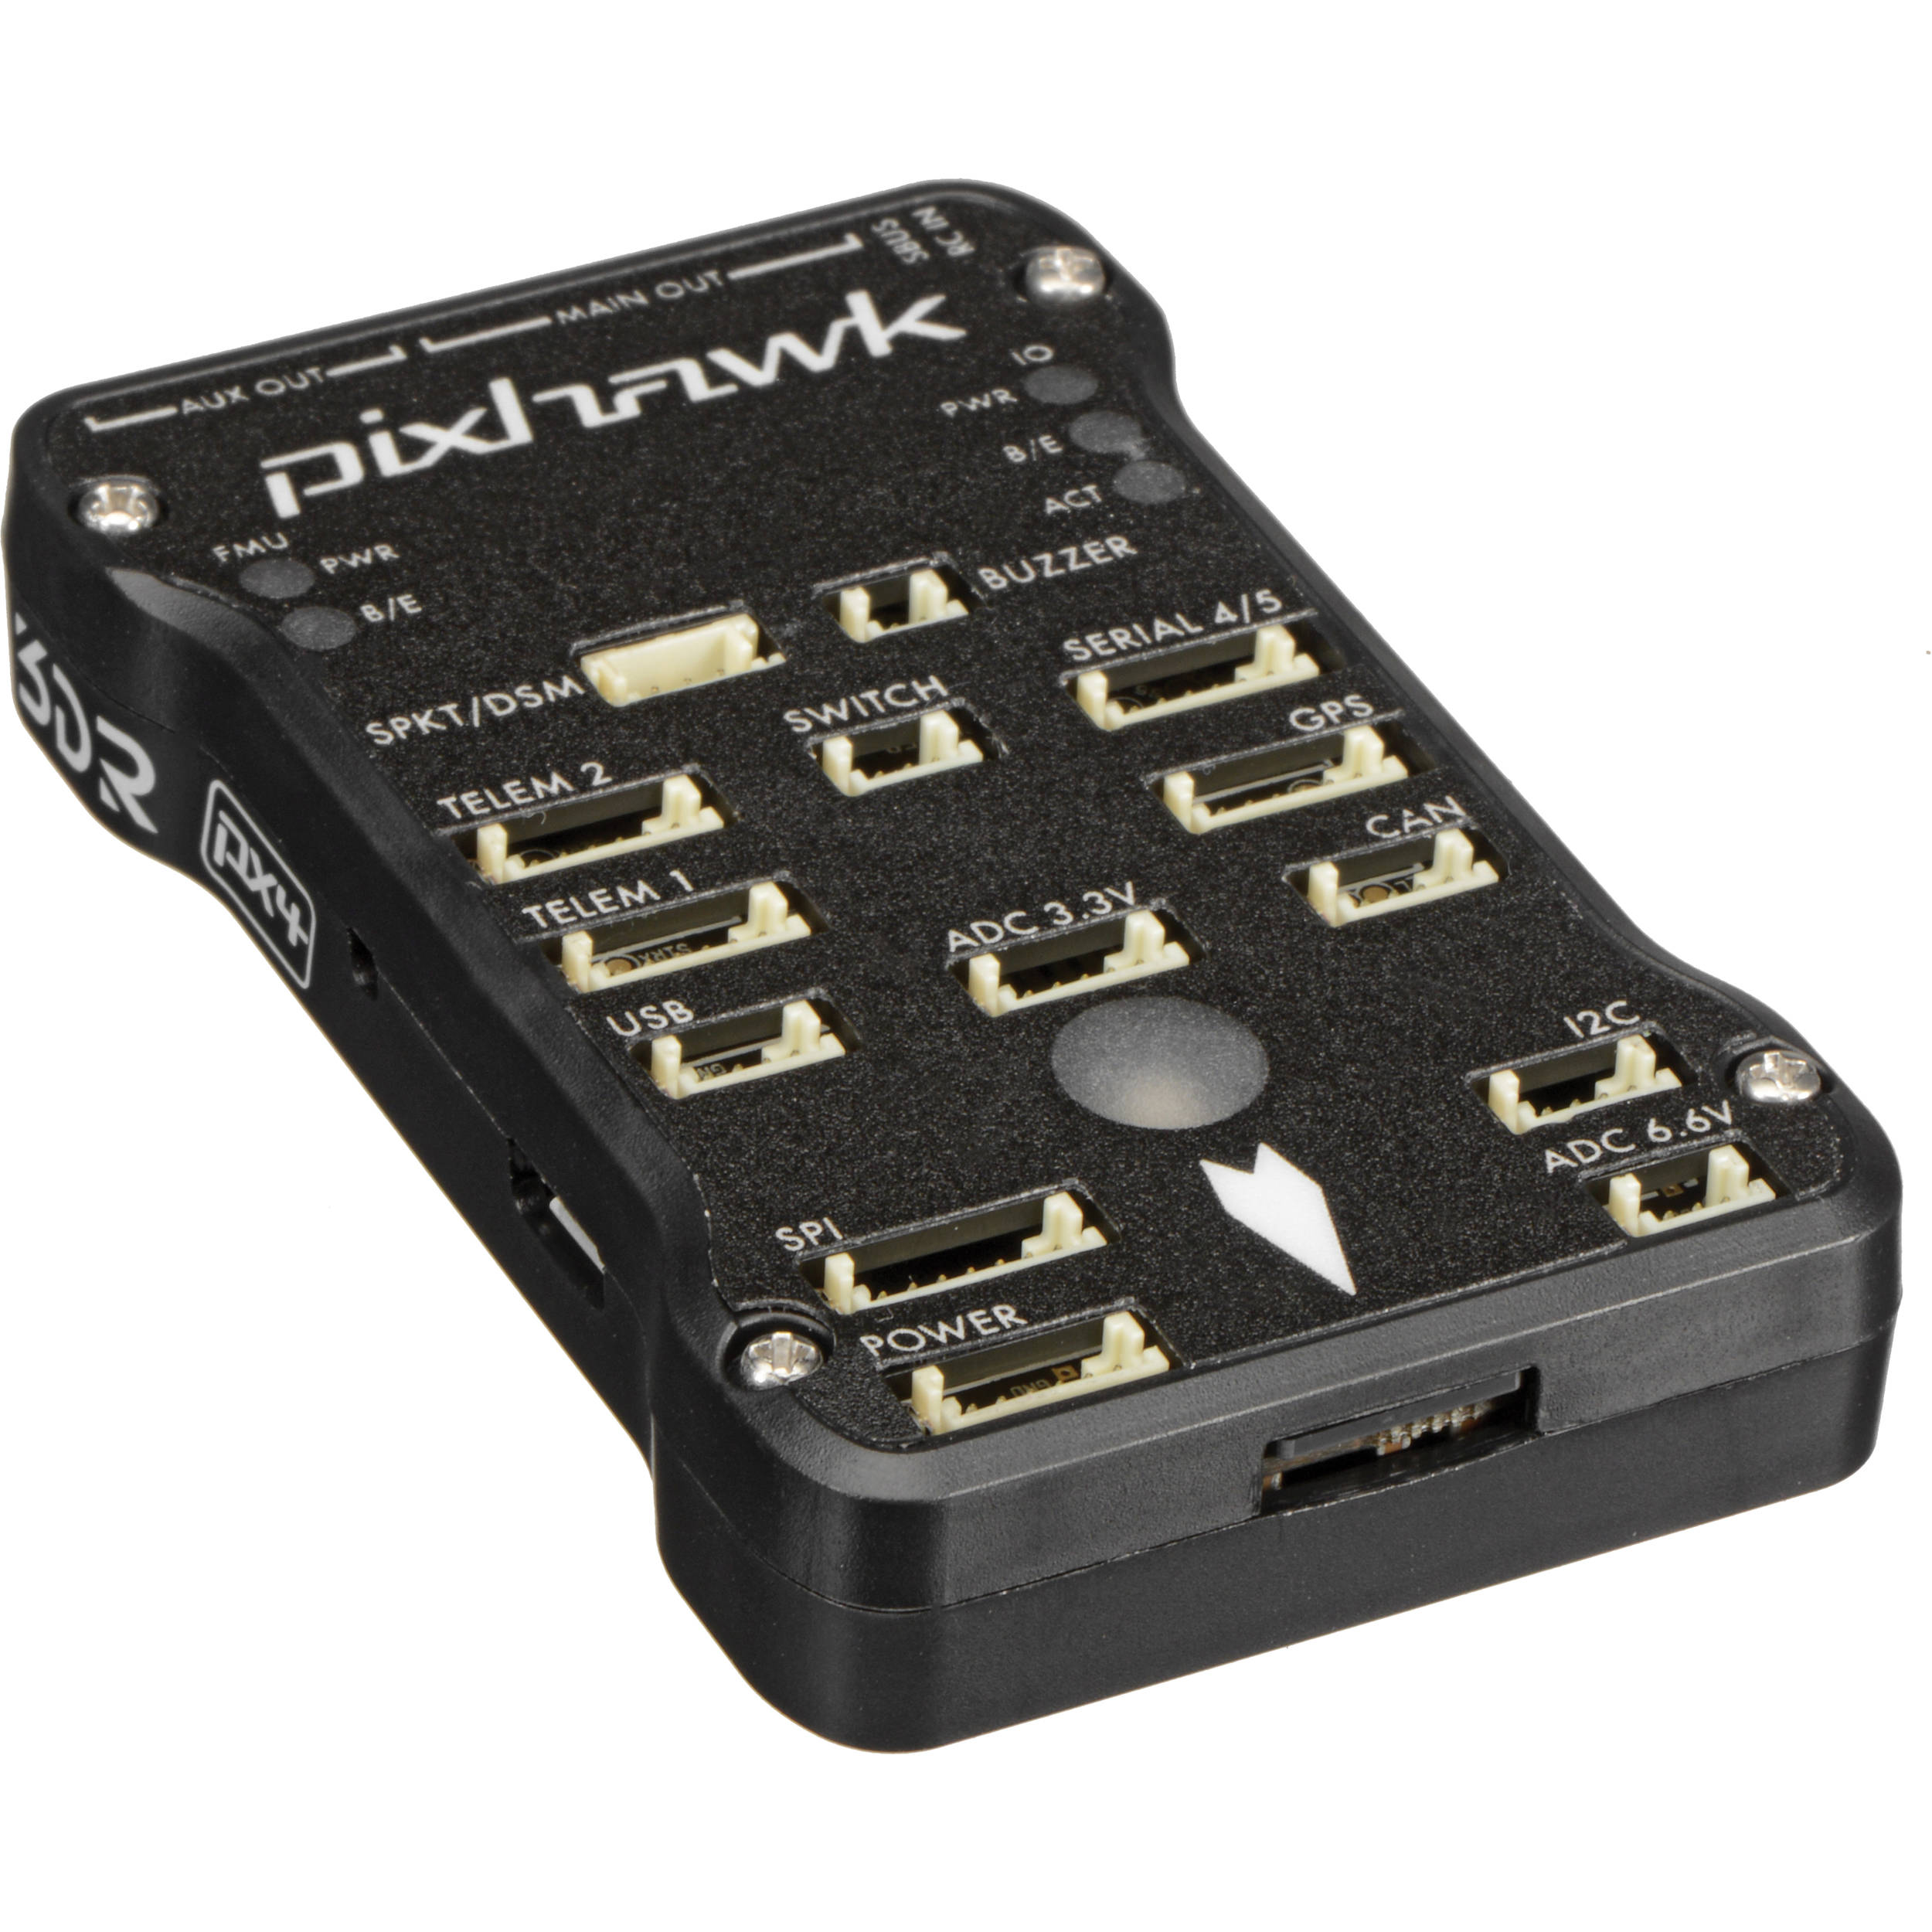
\includegraphics[width=0.3\textwidth] {images/hardware/pixhawk.jpg} 
\caption{Pixhawk Flight-Controller}
\label{fig:pixhawk}
\end{figure}

\begin{figure}[h]
\centering
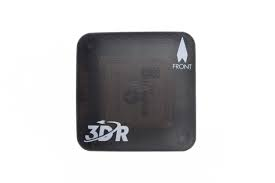
\includegraphics[width=0.3\textwidth] {images/hardware/gps-module.jpg} 
\caption{GPS-Modul für Pixhawk}
\label{fig:gps-module}
\end{figure}

\subsection{Ausbaustufen}

Während des Projekts wurden die Hardware laufend den Bedürfnissen angepasst. Daher gibt es mehrere Prototypen, die für die Versuche genutzt wurden.

\subsubsection{Prototyp 1}

Um das Zusammenspiel der Hardwarekomponenten zu testen und erste Versuche mit dem GPS und den verschiedenen Flugmodi zu sammeln, wurde sehr schnell ein Prototyp gebaut.

\begin{figure}[h]
\centering
\includegraphics[width=0.9\textwidth] {images/hardware/prototype1.jpg} 
\caption{Erster Prototyp ohne Landegestellt und ohne Smartphone}
\label{fig:prototyp-1}
\end{figure}

\subsection{Tests}

Um die Anwendungsmöglichkeiten eines solchen Multicopters auszuloten wurden diverse Experimente durchgeführt um die Leistungsfähigkeit und die Einschränkungen zu testen. 

\subsubsection{Akku Laufzeittest}
Um die maximale Akku Laufzeit zu testen wurde die Drohne ohne zusätzliches Gewicht gestartet, etwa 1.5m über dem Boden schweben gelassen und die Zeit gemessen. Dabei versucht die Drohne die Postion zu halten, bei Abweichung wurde aktiv korrigiert. \\

\begin{tabularx}{\textwidth}{|c|c|X}
\hline
\textbf{Akku} & \textbf{Zuladung}  & \textbf{Laufzeit} \\
3S & keine & 16min 29s\\ \hline 
2x 4S & 500g & 19min\\ \hline 
\end{tabularx}\\

\subsubsection{Tragfähigkeitstests}

Um das maximale Gewicht zu prüfen, das bei einer Präsentation auf unsere Drohnen geladen werden kann, wurden Tests mit dem Zielgewicht von ca. 500g gemacht.Dies Entspricht dem Gewicht einer PET-Flasche eines beliebigen Getränkeherstellers. Ausserdem war auch das Mobiltelefon (ca. 150g) auch auf der Drohne angebracht.  \\

\begin{tabularx}{\textwidth}{|c|c|c|c|X|}
\hline
\textbf{Nutzlast} & \textbf{Akku Typ} & \textbf{Nötige Leistung }& \textbf{Erwartete Flugzeit } & \textbf{Subjektives Flugverhalten }\\
\hline \hline
500g & 3S & ca. 75\%  & n.A. & Ziemlich Träge, mehr Gewicht wäre kritisch\\
\hline
500g & 4S & ca. 45\%  & n.A. & Gewicht kaum Spürbar\\
\hline  
\end{tabularx}\\

Auch mit 3S Akkus scheint es also möglich eine PET-Flasche zu transportieren. 